\chapter{Chapter 7 --- Phases 4 and 5: Noise-Aware ORB, and What
Actually
Helps}\label{chapter-7-phases-4-and-5-noise-aware-orb-and-what-actually-helps}

Chapter 6 established what an online learner cannot survive: the volume
of false positives SZZ invents, amplified by the very mechanism that
corrects class imbalance. It also showed what recovering from that is
worth --- \textbf{+0.040 MCC} --- using the reference labels to remove
exactly the wrong ones.

This chapter answers \textbf{RQ4}: can a learner approximate that repair
\emph{without} the reference, and without sacrificing performance when
the labels are clean?

It reports two pre-registered experiments. \textbf{Phase 4} tests a
train-time false-positive filter and returns a characterised negative.
\textbf{Phase 5}, registered afterwards on data that did not then exist,
tests the confidence-damping alternative --- and its registered
mechanism test, together with one control, produces the chapter's actual
answer, which neither phase was designed to find.

\textbf{The answer is no, and this chapter reports that at full
strength.} The intervention is adoptable --- it does not damage clean
labels --- but no confirmatory test survives multiplicity correction.
This is a \textbf{pre-registered characterised negative}, and the
chapter is organised to explain not merely that it failed but
\emph{why}, because the reason is more informative than a success would
have been.

\section{7.1 Pre-registration, and a registration that was
rewritten}\label{pre-registration-and-a-registration-that-was-rewritten}

\subsection{7.1.1 Why Phase 4 is pre-registered and Phases 1--3 are
not}\label{why-phase-4-is-pre-registered-and-phases-13-are-not}

Phases 1--3 are exploratory. Their hypotheses were formed during
analysis, their test families were defined after seeing the data, and
every result is labelled accordingly, with a conservative global
multiplicity correction applied so that no claim depends on how the
families were drawn.

Phase 4 is different in kind. It proposes a method and asks whether it
works --- a question that invites the analytic flexibility
pre-registration exists to constrain. Its hypotheses, its primary model,
its acceptance bar and its multiplicity correction were therefore
committed to version control \textbf{before the first Phase 4 run}, and
the commit history timestamps that claim independently of this chapter's
narration.

\subsection{7.1.2 The registration was revised once, and the revision is
part of the
record}\label{the-registration-was-revised-once-and-the-revision-is-part-of-the-record}

The original registration made a \textbf{false-negative rescue}
mechanism the headline: when the ensemble confidently disagrees with a
clean label, train the commit as a provisional positive. That design
followed directly from the starvation hypothesis Phase 4 was planned
under.

Chapter 6 refuted that hypothesis. Restoring genuinely missing defect
labels is \emph{equivalent to no repair} (TOST \emph{p} = 0.0008). A
mechanism that manufactures positives therefore targets an error shown
to cost nothing --- and worse, every incorrect rescue manufactures
exactly the error type Chapter 6 showed to be costly.

Because Phase 4 had produced \textbf{zero results} at that point, the
registration was rewritten and re-committed. \textbf{That is the only
moment at which revising a pre-registration is legitimate}: before any
outcome is visible. Revising afterwards is the practice pre-registration
exists to prevent, and the distinction between the two is entirely a
matter of timing, which is why the timing is recorded rather than
asserted.

The rescue mechanism was not discarded. It was \textbf{demoted to a
mechanism probe carrying a predicted sign}, so that it would test
Chapter 6's account rather than merely be excluded by it.

\subsection{7.1.3 The registered tests}\label{the-registered-tests}

\begin{longtable}[]{@{}
  >{\raggedright\arraybackslash}p{(\linewidth - 4\tabcolsep) * \real{0.3333}}
  >{\raggedright\arraybackslash}p{(\linewidth - 4\tabcolsep) * \real{0.3333}}
  >{\raggedright\arraybackslash}p{(\linewidth - 4\tabcolsep) * \real{0.3333}}@{}}
\toprule\noalign{}
\begin{minipage}[b]{\linewidth}\raggedright
Tag
\end{minipage} & \begin{minipage}[b]{\linewidth}\raggedright
Test
\end{minipage} & \begin{minipage}[b]{\linewidth}\raggedright
Prediction
\end{minipage} \\
\midrule\noalign{}
\endhead
\bottomrule\noalign{}
\endlastfoot
\textbf{ND} & Filter vs baseline on reference labels & \textbf{No
significant drop} (TOST, \ensuremath{\pm}0.02). The acceptance bar \\
\textbf{H1} & Filter beats baseline on B-SZZ & Positive (6,565 false
positives --- the most available) \\
\textbf{H2a/b} & Filter beats baseline on MA-SZZ and AG-SZZ & Positive
(5,030 and 4,786) \\
\textbf{H3} & Benefit rank-correlates with each variant's false-positive
count & \ensuremath{\rho} \textgreater{} 0, one-sided \\
\textbf{MP} & Rescue vs baseline on every SZZ source & \textbf{\ensuremath{\leq} 0} on
all six \\
\textbf{R1} & \ensuremath{\lambda} self-antagonism arm & \texttt{suppress} underperforms
\texttt{observed} \\
\end{longtable}

\textbf{H3 is the sharpest test in the chapter}, and it exists because
of Chapter 6's error-matched control. If the benefit is driven by
false-positive \emph{volume}, it should track how many false positives
each source contains --- a predicted ordering over six variants whose
counts were fixed in advance (6565, 5030, 4786, 4531, 2316, 1665). An
ordering is far harder to satisfy by chance than a binary comparison.

\textbf{ND is the acceptance bar, not H1.} A filter that wins on noisy
labels and damages clean ones is not deployable, because a practitioner
cannot know in advance which case they are in.

\section{7.2 Design}\label{design}

\subsection{7.2.1 The intervention}\label{the-intervention}

\texttt{FPFilterORB} extends ORB with train-time false-positive
suppression. A defect-labelled arrival that the ensemble confidently
contradicts is treated as a suspected SZZ false positive: trained at
weight \ensuremath{\varepsilon} (with \ensuremath{\varepsilon} = 0 discarding it) and excluded from the boost.
\textbf{Clean-labelled arrivals are untouched}, since Chapter 6 showed
that intervening on the negative side recovers nothing.

\subsection{7.2.2 Two decision rules, and why the obvious one
fails}\label{two-decision-rules-and-why-the-obvious-one-fails}

The natural rule --- and the one originally specified --- is a running
quantile: suppress a positive whose probability falls in the lowest
\emph{q} of recently delivered positives. It requires no calibration,
which is its appeal.

\textbf{Measured on this corpus that rule is degenerate.} The ensemble's
members agree almost completely, so the predicted probability is bimodal
at 0 and 1, and the 10th percentile of a trailing window is
\textbf{0.0000 in nearly every segment of every stream}. A strict
comparison against a threshold of zero can never fire: on opennlp/B-SZZ
it suppressed \textbf{0 of 75} positive arrivals. The rule was not wrong
in conception; it was wrong in its comparison operator, and a non-strict
comparison repairs it.

The alternative is a fixed threshold \ensuremath{\tau}. \S{}7.4.1 shows it fails for a
deeper reason.

\begin{verbatim}
FPFilterORB.learn_one(x, y):
    if y == 0:
        ORB.learn_one(x, y);  return          # negatives untouched

    p1  \ensuremath{\leftarrow} ensemble_probability(x)
    thr \ensuremath{\leftarrow} \ensuremath{\tau}                    if mode = fixed
          quantile(window, q)  if mode = quantile and |window| \ensuremath{\geq} min_pos
          \ensuremath{\bot}                    otherwise      # inert during warm-up
    suspect \ensuremath{\leftarrow} (thr \ensuremath{\neq} \ensuremath{\bot}) and (p1 < thr  if fixed  else  p1 \ensuremath{\leq} thr)
    window.append(p1)

    if suspect:
        if rate_update = "observed":
            r\ensuremath{_1} \ensuremath{\leftarrow} decay\ensuremath{\cdot}r\ensuremath{_1} + (1\ensuremath{-}decay)\ensuremath{\cdot}1       # distrust the LABEL, not the class rate
        if \ensuremath{\varepsilon} > 0:
            k ~ Poisson(\ensuremath{\varepsilon});  update_members(x, 1, k)
        return                                 # no boost, no full-weight update

    ORB.learn_one(x, y)
\end{verbatim}

\textbf{Complexity.} One additional ensemble forward pass per
defect-labelled arrival and one quantile over a bounded window, so
\emph{O}(\emph{M} + log \emph{W}) per positive with \emph{M} ensemble
members and window \emph{W}, against ORB's \emph{O}(\emph{M}\ensuremath{\cdot}\ensuremath{\lambda}) update.
Since positives are 8.5\% of arrivals and \ensuremath{\lambda} routinely exceeds 20, the
filter's cost is negligible.

\textbf{Warm-up is counted in positive labels, not arrivals.} Positives
are what is scarce: under realistic latency some projects deliver fewer
than 30 across an entire stream, and a quantile over an empty window is
undefined. Below \texttt{min\_pos} the filter is inert and the model is
plain ORB --- the safe direction.

\subsection{7.2.3 The registered risk: \ensuremath{\lambda}
self-antagonism}\label{the-registered-risk-ux3bb-self-antagonism}

Chapter 6 measured ORB's oversampling rate to be a near-perfect inverse
of delivered defect-label supply (\ensuremath{\rho} = \ensuremath{-}1.000), and the mechanism is
explicit in the update: \ensuremath{\lambda}\ensuremath{_1} = (1 \ensuremath{-} r\ensuremath{_1})/r\ensuremath{_1}. \textbf{Every positive this
filter suppresses therefore raises \ensuremath{\lambda} for the positives that survive it.}
The filter works against the machinery it is bolted onto.

The \texttt{rate\_update} switch controls whether it does:

\begin{itemize}
\tightlist
\item
  \textbf{\texttt{observed}} --- r\ensuremath{_1} is updated as though the label had
  been accepted. Suppressing a label expresses distrust of \emph{that
  label} without telling the ensemble the defect class is rarer than it
  is. \ensuremath{\lambda} is left alone.
\item
  \textbf{\texttt{suppress}} --- the arrival is skipped entirely, r\ensuremath{_1}
  drifts down, \ensuremath{\lambda} rises.
\end{itemize}

\textbf{Registered prediction: \texttt{suppress} underperforms
\texttt{observed}, with the gap widening as filter rate rises.} A second
risk --- that a suppressed positive is never learned, so its probability
stays low and it is suppressed again --- is instrumented rather than
assumed: every decision is traced.

\section{7.3 Experimental setup}\label{experimental-setup}

\textbf{Models.} OOB and ORB as baselines; \texttt{NA(fp\_filter)} as
the registered primary; \texttt{NA(fp\_filter/suppress)} as the R1 arm,
carrying identical hyperparameters with only the switch flipped;
\texttt{NA(damp)}, the prior confidence-damping defence, for comparison;
\texttt{NA(rescue)} as the MP probe.

A composed \texttt{NA(fp\_filter+damp)} arm appeared in the first draft
of the registration but was \textbf{never implemented} --- the
placeholder returned a duplicate of the primary, which would have
reported one model under two names and made the ablation look richer
than it is. It was dropped before any Phase 4 run, at the same moment
and for the same reason the registration itself could legitimately be
revised.

\textbf{Conditions.} Reference labels (the ND gate), all six SZZ
variants, and a 20\% injected-noise condition bridging to Chapter 6.

\textbf{Held-out projects.} \texttt{commons-scxml}, \texttt{opennlp} and
\texttt{commons-math} are excluded from every reported number.
Hyperparameters were chosen by looking at them, so including them would
leak the tuning set into the results. Reporting is therefore on
\textbf{18 projects}.

\textbf{Statistics.} Project-paired Wilcoxon on \texttt{mcc\_avg},
Hodges--Lehmann with bootstrap interval, matched-pairs rank-biserial,
Holm within the registered family. Both estimators recorded.

\section{7.4 Results}\label{results}

\subsection{7.4.1 Tuning, and what the acceptance bar
caught}\label{tuning-and-what-the-acceptance-bar-caught}

Forty-two configurations were evaluated on the held-out projects under a
selection rule declared before the sweep: apply the ND gate
\textbf{first}, then maximise gain on B-SZZ, then prefer the more
conservative filter. \texttt{rate\_update} was deliberately \textbf{not}
tuned --- it is the R1 arm, and optimising it would convert a registered
prediction into a fit.

\textbf{Twenty-four configurations passed the gate, and every one of
them uses the quantile rule.} Every fixed-threshold configuration
failed, several catastrophically: on the reference arm, where every
positive label is correct and there is nothing to remove, \ensuremath{\tau} = 0.35
suppressed 57\% of defect labels and cost \textbf{\ensuremath{-}0.0989} MCC.

\begin{quote}
\textbf{The reason generalises well beyond this model.} A fixed
confidence threshold suppresses however many positives the model happens
to be unsure about, with no reference to how many false positives the
source actually contains. It cannot distinguish \emph{``this label is
probably wrong''} from \emph{``my model has not learned this pattern
yet.''} A quantile rule removes about \emph{q} by construction, so its
worst case is bounded. \textbf{An intervention on scarce labels must be
bounded in size, not in confidence.}
\end{quote}

The frozen configuration is quantile with \emph{q} = 0.30, \ensuremath{\varepsilon} = 0.1,
\texttt{min\_pos} = 30, \texttt{rate\_update} = \texttt{observed}.
Extending the sweep to \emph{q} = 0.40 and 0.50 lowered the B-SZZ gain
to 0.0402 and 0.0288, confirming \emph{q} = 0.30 as an interior optimum
rather than a grid edge.

\subsection{7.4.2 The registered verdict}\label{the-registered-verdict}

Eighteen reporting projects.

\begin{longtable}[]{@{}
  >{\raggedright\arraybackslash}p{(\linewidth - 10\tabcolsep) * \real{0.1667}}
  >{\raggedright\arraybackslash}p{(\linewidth - 10\tabcolsep) * \real{0.1667}}
  >{\raggedright\arraybackslash}p{(\linewidth - 10\tabcolsep) * \real{0.1667}}
  >{\raggedright\arraybackslash}p{(\linewidth - 10\tabcolsep) * \real{0.1667}}
  >{\raggedright\arraybackslash}p{(\linewidth - 10\tabcolsep) * \real{0.1667}}
  >{\raggedright\arraybackslash}p{(\linewidth - 10\tabcolsep) * \real{0.1667}}@{}}
\toprule\noalign{}
\begin{minipage}[b]{\linewidth}\raggedright
Test
\end{minipage} & \begin{minipage}[b]{\linewidth}\raggedright
HL
\end{minipage} & \begin{minipage}[b]{\linewidth}\raggedright
95\% CI
\end{minipage} & \begin{minipage}[b]{\linewidth}\raggedright
Projects
\end{minipage} & \begin{minipage}[b]{\linewidth}\raggedright
\emph{p}
\end{minipage} & \begin{minipage}[b]{\linewidth}\raggedright
\textbf{Holm}
\end{minipage} \\
\midrule\noalign{}
\endhead
\bottomrule\noalign{}
\endlastfoot
\textbf{ND} --- non-degradation on reference labels & \ensuremath{-}0.0001 &
{[}\ensuremath{-}0.0091, +0.0081{]} & 5/18 & 0.807 & \textbf{PASS} \\
H1 --- filter beats baseline on B-SZZ & +0.0166 & {[}+0.0009, +0.0328{]}
& 12/18 & 0.054 & 0.215 x \\
H2a --- on MA-SZZ & +0.0110 & {[}\ensuremath{-}0.0005, +0.0235{]} & 13/18 & 0.074 &
0.221 x \\
H2b --- on AG-SZZ & +0.0072 & {[}\ensuremath{-}0.0075, +0.0221{]} & 12/18 & 0.246 &
0.492 x \\
H3 --- benefit tracks false-positive count & \ensuremath{\rho} = 0.714 & --- & 6
variants & 0.055 & x \\
\end{longtable}

\textbf{The gate passes; nothing else does.}

\begin{figure}
\centering
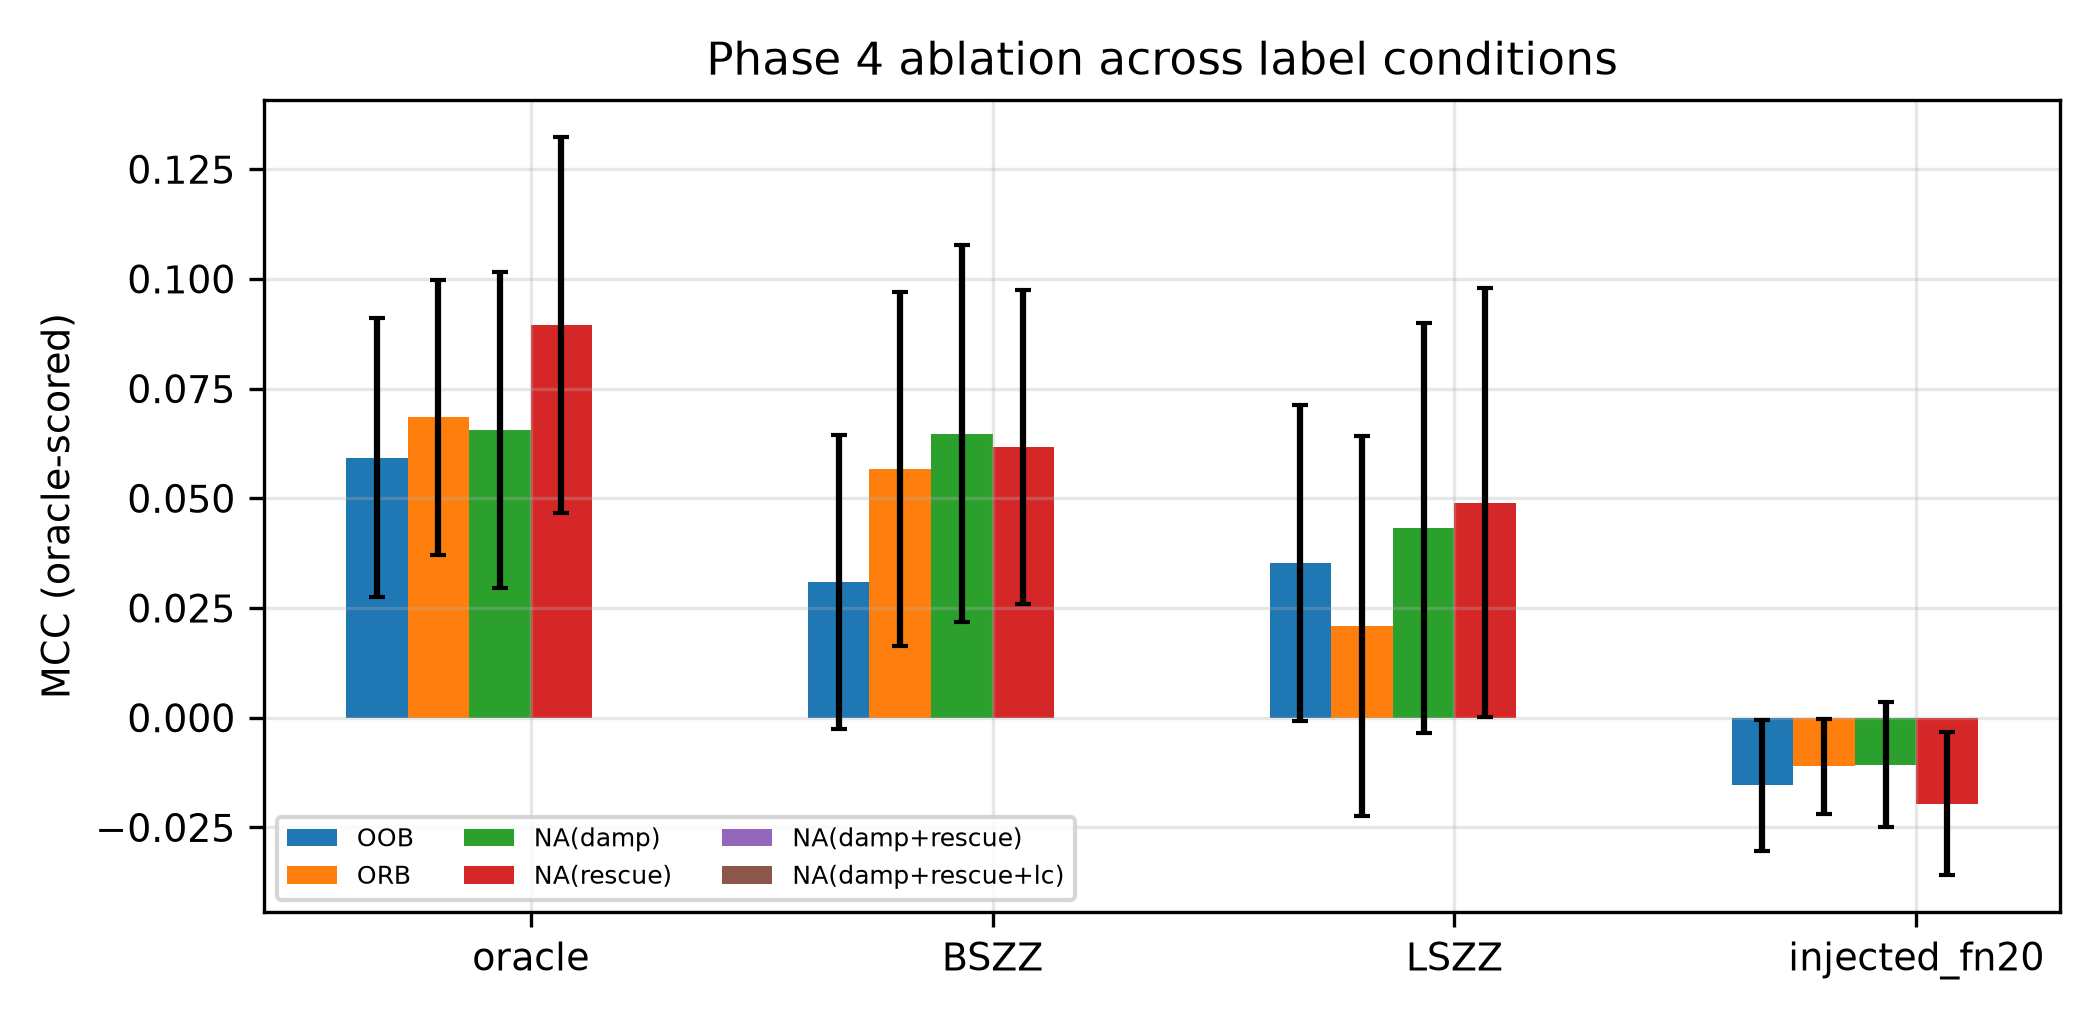
\includegraphics[width=\linewidth,keepaspectratio]{reports/figures/fig_p4_ablation.png}
\label{fig:fig_p4_ablation}
\caption{Phase 4 ablation across models and label conditions}
\end{figure}

\textbf{Figure 7.1 --- Reading the figure.} Six models across six label
conditions, 18 reporting projects, error bars 95\% intervals. Every
noise-aware variant sits above the ORB baseline on every SZZ source, and
the intervals overlap heavily --- which is the visual form of
``consistent in direction, not significant after correction''. Note that
\texttt{NA(damp)} (green), the arm the re-registration demoted, is the
tallest bar on B-SZZ, MA-SZZ and AG-SZZ.

\begin{figure}
\centering
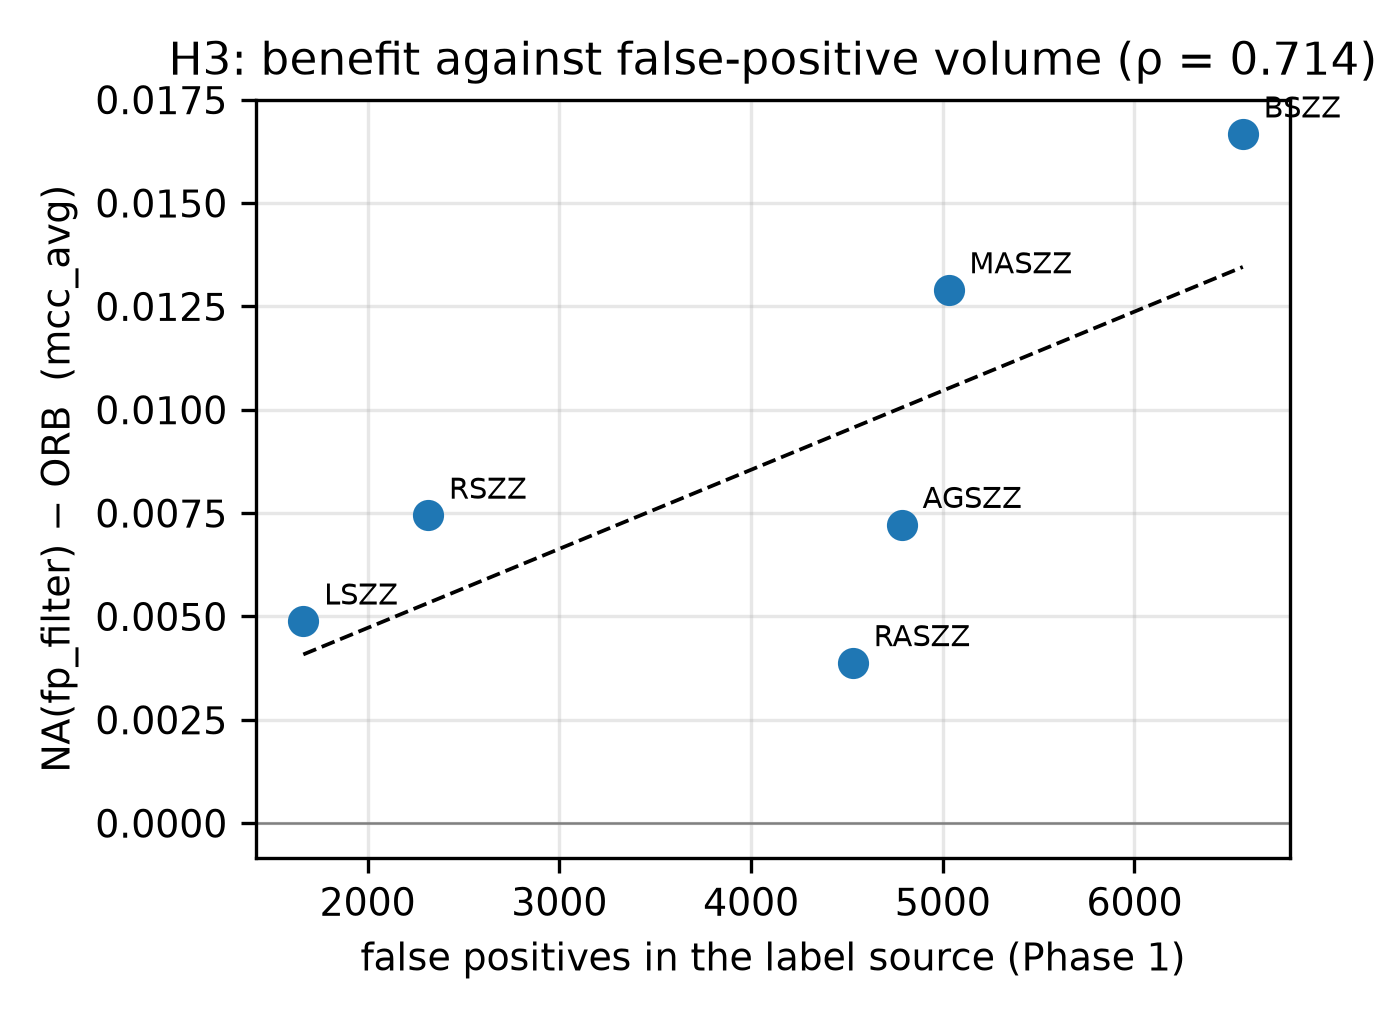
\includegraphics[width=\linewidth,keepaspectratio]{reports/figures/fig_p4_h3_volume.png}
\label{fig:fig_p4_h3_volume}
\caption{H3 --- benefit against each source's false-positive count}
\end{figure}

\textbf{Figure 7.2 --- Reading the figure.} Each point is one SZZ
variant, positioned by how many false positives Chapter 4 measured in it
and by the filter's mean gain over the baseline. The dashed line is the
fitted trend. \textbf{The ordering is broadly as predicted} --- the gain
rises with false-positive volume --- but with six variants and one
inversion (RA-SZZ), \ensuremath{\rho} = 0.714 does not reach significance.

\begin{figure}
\centering
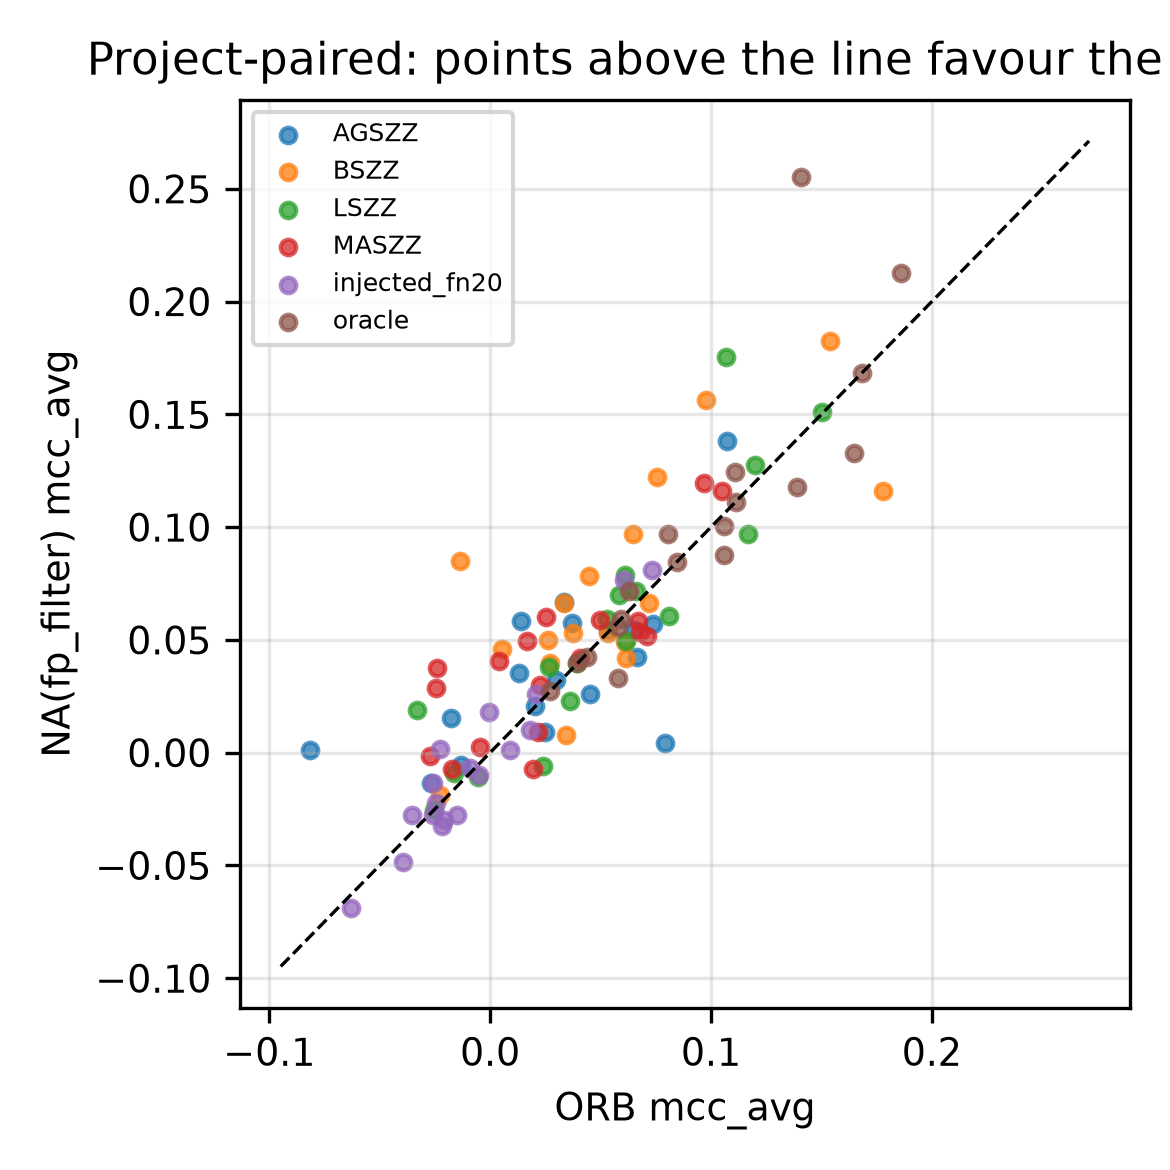
\includegraphics[width=\linewidth,keepaspectratio]{reports/figures/fig_p4_paired_scatter.png}
\label{fig:fig_p4_paired_scatter}
\caption{Project-paired comparison of the filter against the baseline}
\end{figure}

\textbf{Figure 7.3 --- Reading the figure.} One point per project per
condition; points above the dashed diagonal are projects where the
filter beat the baseline. The cloud sits slightly above the line and
straddles it --- a majority of projects improve, not enough of them to
establish the effect. Every confirmatory test points in the predicted
direction and not one survives correction.

The honest reading is narrow. The filter is \textbf{adoptable} --- it
does not damage clean labels, which is the property that gates
deployment --- but it is \textbf{not demonstrated to work}. Four
independent tests agreeing in direction is worth a sentence; it is not a
result, and this thesis does not treat it as one. H1's interval barely
excludes zero and its raw \emph{p} of 0.054 would not have survived even
without correction.

\textbf{The hold-out protocol paid for itself.} On the three tuning
projects the filter gained \textbf{+0.045} on B-SZZ. On the 18 reporting
projects it gains \textbf{+0.017} --- an optimism factor of
\textbf{2.7\ensuremath{\times}}. Had the hyperparameters been selected on the reporting
set, this chapter would have claimed an effect nearly three times its
real size, and would have been wrong.

\subsection{7.4.3 The mechanism probe was refuted, 0 for
6}\label{the-mechanism-probe-was-refuted-0-for-6}

Rescue was registered with an explicit prediction that it would be
\textbf{at or below zero} on every SZZ source. It is \textbf{positive on
all six}:

\begin{longtable}[]{@{}lllll@{}}
\toprule\noalign{}
Source & Rescue \ensuremath{-} baseline & 95\% CI & Projects & \emph{p} \\
\midrule\noalign{}
\endhead
\bottomrule\noalign{}
\endlastfoot
L-SZZ & \textbf{+0.0166} & {[}+0.0057, +0.0289{]} & 13/18 & 0.006 \\
MA-SZZ & \textbf{+0.0142} & {[}+0.0013, +0.0266{]} & 12/18 & 0.027 \\
AG-SZZ & +0.0117 & {[}\ensuremath{-}0.0007, +0.0270{]} & 13/18 & 0.090 \\
B-SZZ & \textbf{+0.0116} & {[}+0.0033, +0.0262{]} & 13/18 & 0.024 \\
R-SZZ & +0.0068 & {[}\ensuremath{-}0.0033, +0.0202{]} & 12/18 & 0.246 \\
RA-SZZ & +0.0002 & {[}\ensuremath{-}0.0164, +0.0213{]} & 8/18 & 1.000 \\
\end{longtable}

The registration stated that if rescue helped, the mechanism account
would need revision. \textbf{It helps, and the revision is owed.}

\textbf{The candidate reconciliation, and why it is not yet a claim.}
Chapter 6 restored the \emph{reference-known} missing positives; rescue
adds \emph{model-confident} ones. These are different sets --- rescue is
closer to self-training on high-confidence commits than to label
correction. So ``restoring what SZZ missed recovers nothing'' and
``adding confidently-predicted defects helps'' are not contradictory,
\textbf{provided} the benefit comes from label \emph{supply} rather than
label \emph{accuracy}.

That explanation was tested directly. The Spearman correlation between a
condition's delivered positive supply and the filter-minus-rescue
advantage is \textbf{\ensuremath{\rho} = +0.357, \emph{p} = 0.385}. \textbf{The supply
account is not supported}, and it is recorded here as an open question
rather than presented as an explanation.

\subsection{7.4.4 R1: a clean null in both
directions}\label{r1-a-clean-null-in-both-directions}

\begin{longtable}[]{@{}llll@{}}
\toprule\noalign{}
Condition & observed \ensuremath{-} suppress & 95\% CI & \emph{p} \\
\midrule\noalign{}
\endhead
\bottomrule\noalign{}
\endlastfoot
B-SZZ & \ensuremath{-}0.0016 & {[}\ensuremath{-}0.0075, +0.0045{]} & 0.61 \\
Reference & +0.0002 & {[}\ensuremath{-}0.0018, +0.0031{]} & 0.51 \\
\end{longtable}

The registered prediction is not supported, and neither is its converse.
\ensuremath{\lambda} \emph{does} rise when positives are suppressed --- the coupling is
real and was measured at \ensuremath{\rho} = \ensuremath{-}1.000 --- but at this filter rate it has
no detectable effect on performance. The trace confirms the feedback
loop exists: the two settings produce \emph{different filter rates on
identical inputs}. It simply does not matter at this magnitude.

\subsection{7.4.5 An uncomfortable finding, reported rather than
smoothed}\label{an-uncomfortable-finding-reported-rather-than-smoothed}

The prior confidence-damping arm --- the one the re-registration demoted
--- \textbf{outperforms the new primary on six of eight conditions},
including B-SZZ (0.0874 against the baseline's 0.0551).

Because damping was not the registered primary, every such contrast is
exploratory. Corrected across the 21 exploratory contrasts, only
damping-beats-baseline on B-SZZ survives global Holm: +0.0329, CI
{[}+0.0194, +0.0456{]}, 15/18, \emph{p} = 0.0040. \textbf{The defensible
statement is that damping leads numerically and is established on one
label source.}

The re-registration was correctly motivated by Chapter 6 and correctly
timed before any run, and it still bet on the wrong arm. The commit
history records this either way, so the thesis states it.

\section{7.5 Phase 5 --- the registered follow-up, and what it
overturned}\label{phase-5-the-registered-follow-up-and-what-it-overturned}

Phase 4's exploratory analysis left one loose end. \texttt{NA(damp)} ---
the arm the re-registration demoted --- outperformed the registered
primary on six of eight conditions. That observation was generated by
the Phase 4 data, so testing it there would confirm a hypothesis on the
sample that produced it.

Phase 5 therefore registers the damping hypothesis and tests it on data
that did not exist at registration time: the \textbf{noise-injection
grid} of four profiles crossed with six doses, which Chapter 6 ran with
plain ORB only and Phase 4 touched at a single dose. The registration
was committed with no results in the commit; the run follows it in the
history.

\subsection{7.5.1 The registered
scorecard}\label{the-registered-scorecard}

34,560 records --- 18 reporting projects \ensuremath{\times} 10 seeds \ensuremath{\times} 4 profiles \ensuremath{\times} 6
doses \ensuremath{\times} 2 latency arms \ensuremath{\times} 4 models.

\begin{longtable}[]{@{}
  >{\raggedright\arraybackslash}p{(\linewidth - 6\tabcolsep) * \real{0.2500}}
  >{\raggedright\arraybackslash}p{(\linewidth - 6\tabcolsep) * \real{0.2500}}
  >{\raggedright\arraybackslash}p{(\linewidth - 6\tabcolsep) * \real{0.2500}}
  >{\raggedright\arraybackslash}p{(\linewidth - 6\tabcolsep) * \real{0.2500}}@{}}
\toprule\noalign{}
\begin{minipage}[b]{\linewidth}\raggedright
Test
\end{minipage} & \begin{minipage}[b]{\linewidth}\raggedright
Prediction
\end{minipage} & \begin{minipage}[b]{\linewidth}\raggedright
Result
\end{minipage} & \begin{minipage}[b]{\linewidth}\raggedright
\end{minipage} \\
\midrule\noalign{}
\endhead
\bottomrule\noalign{}
\endlastfoot
\textbf{H1} damp \textgreater{} ORB, FP-heavy & positive &
\textbf{+0.0168} {[}+0.0092, +0.0272{]}, 15/18, Holm \textbf{0.0021} &
\textbf{pass} \\
\textbf{H4} damp \textgreater{} filter, FP-heavy & positive &
\textbf{+0.0081} {[}+0.0022, +0.0141{]}, 15/18, Holm \textbf{0.018} &
\textbf{pass} \\
\textbf{ND} no degradation & no drop & \textbf{+0.0193} {[}+0.0092,
+0.0299{]}, Holm 0.0039 & \textbf{pass} \\
\textbf{H3} FN-heavy advantage \textgreater{} FP-heavy & positive &
\textbf{\ensuremath{-}0.0217} {[}\ensuremath{-}0.0341, \ensuremath{-}0.0118{]}, \textbf{2/18}, Holm
\textbf{0.0021} & \textbf{fail} refuted, opposite direction \\
\textbf{H2} advantage grows with dose & \ensuremath{\rho} \textgreater{} 0 & \ensuremath{\rho} =
\textbf{\ensuremath{-}0.486}, \emph{p} = 0.84 & \textbf{fail} \\
\end{longtable}

Two pass; two fail --- and \textbf{the two that fail are the ones about
the mechanism.}

H4 is worth isolating, because it settles a question Phase 4 could only
speculate about: \textbf{down-weighting a suspect label beats discarding
it}, by +0.0081 with 15 of 18 projects agreeing. Under the label
scarcity that verification latency imposes, the cheaper error is to keep
a doubtful label at reduced influence rather than to throw it away.

\textbf{A defect in the registration, recorded rather than quietly
repaired.} The ND gate was registered as a TOST for \emph{equivalence}
at \ensuremath{\pm}0.02. It returns ``not equivalent'' --- because damping is
\textbf{better} than the baseline by more than the margin, not worse.
The gate's intent is met decisively; the registered statistic was simply
the wrong one, since the correct test for a non-degradation gate is
\textbf{non-inferiority}, one-sided against \ensuremath{-}margin. The direction is
unambiguous either way, so nothing is rescued by substituting it, and
the mis-specification is reported because it was registered.

\subsection{7.5.2 H3's refutation is the informative
half}\label{h3s-refutation-is-the-informative-half}

H3 predicted that damping should help \emph{most} under FN-heavy noise
at doses \ensuremath{\geq} 0.20 --- the regime where Chapter 6 measured the stream
retaining no genuine defect labels while still carrying roughly 204
positive labels, \textbf{every one of them false}. If damping suppresses
the influence of wrong positives, an entirely wrong positive stream is
where it should shine.

It helps \textbf{least} there, significantly so, with only 2 of 18
projects moving the predicted way. Two candidate explanations, neither
tested:

\begin{enumerate}
\def\labelenumi{\arabic{enumi}.}
\tightlist
\item
  \textbf{No discriminative signal.} Confidence damping needs a
  \emph{mixture} of correct and incorrect positives to tell them apart.
  When every positive is wrong there is no reference class for what a
  trustworthy positive looks like.
\item
  \textbf{A lower ceiling.} Every model scores \ensuremath{\approx} 0.02 under FN-heavy
  against \ensuremath{\approx} 0.05 under FP-heavy, leaving less room for any advantage.
  The relative gap (1.19\ensuremath{\times} against 1.57\ensuremath{\times}) suggests this contributes
  without being sufficient.
\end{enumerate}

\subsection{7.5.3 The control that explains H1
away}\label{the-control-that-explains-h1-away}

ORB is OOB plus a prediction-bias boost; \texttt{NA(damp)} is ORB plus
confidence damping. Including plain OOB in the grid separates the two
contributions:

\begin{longtable}[]{@{}
  >{\raggedright\arraybackslash}p{(\linewidth - 6\tabcolsep) * \real{0.2500}}
  >{\raggedright\arraybackslash}p{(\linewidth - 6\tabcolsep) * \real{0.2500}}
  >{\raggedright\arraybackslash}p{(\linewidth - 6\tabcolsep) * \real{0.2500}}
  >{\raggedright\arraybackslash}p{(\linewidth - 6\tabcolsep) * \real{0.2500}}@{}}
\toprule\noalign{}
\begin{minipage}[b]{\linewidth}\raggedright
Profile
\end{minipage} & \begin{minipage}[b]{\linewidth}\raggedright
NA(damp) \ensuremath{-} ORB
\end{minipage} & \begin{minipage}[b]{\linewidth}\raggedright
\textbf{OOB \ensuremath{-} ORB}
\end{minipage} & \begin{minipage}[b]{\linewidth}\raggedright
\textbf{NA(damp) \ensuremath{-} OOB}
\end{minipage} \\
\midrule\noalign{}
\endhead
\bottomrule\noalign{}
\endlastfoot
FP-heavy & +0.0168 (Holm 0.0047) & \textbf{+0.0172 --- 18/18, Holm
0.0001} & +0.0019 (9/18, Holm 1.00) \\
symmetric & +0.0181 (Holm 0.0014) & \textbf{+0.0199 --- 17/18, Holm
0.0002} & +0.0005 (8/18, Holm 1.00) \\
mid & +0.0139 (Holm 0.0023) & \textbf{+0.0139 --- 15/18, Holm 0.0026} &
+0.0020 (10/18, Holm 1.00) \\
FN-heavy & +0.0028 (n.s.) & +0.0075 (15/18, Holm 0.109) & \ensuremath{-}0.0050 (6/18,
Holm 1.00) \\
\end{longtable}

\begin{quote}
\textbf{Damping adds nothing over simply not boosting.} Against plain
OOB it is a coin flip in every profile --- 8 to 10 wins out of 18, every
interval spanning zero, every corrected \emph{p} at 1.000. The entire H1
effect is reproduced by removing the boost and adding no noise-awareness
at all.
\end{quote}

\textbf{H1 passes and the control explains it away.} This is what
pre-registration is for: the registered effect test confirmed the
effect, the registered mechanism test refuted the explanation, and a
control identified the real cause. Had damping been promoted on Phase
4's exploratory evidence, the thesis would have reported a noise-aware
method that works --- and been wrong about why, in a way no amount of
additional significance would have caught.

\subsection{7.5.4 What Phase 5
establishes}\label{what-phase-5-establishes}

\textbf{ORB's prediction-bias boost is what costs performance under
label noise.} Eighteen of eighteen projects on the FP-heavy profile ---
the strongest single result in Phases 4 and 5. It is independent
confirmation of Chapter 6's amplification account, obtained by
\textbf{intervention} rather than by measuring the oversampling rate,
and the two lines of evidence are methodologically independent.

It is also consistent with, though not established by, the clean-label
comparison: on reference labels in Phase 4 the same contrast was +0.0050
(\emph{p} = 0.47, not significant) against +0.0172 under injected
FP-heavy noise here. \textbf{The boost appears roughly neutral on
correct labels and harmful on incorrect ones}, which is what the
amplification account predicts. The interaction was not formally tested
and is not claimed.

\section{7.6 Discussion --- answering
RQ4}\label{discussion-answering-rq4}

\textbf{Can a learner recover performance lost to SZZ noise without
reference labels?} Not demonstrably, on this corpus, with this
intervention.

\begin{longtable}[]{@{}
  >{\raggedright\arraybackslash}p{(\linewidth - 2\tabcolsep) * \real{0.5000}}
  >{\raggedright\arraybackslash}p{(\linewidth - 2\tabcolsep) * \real{0.5000}}@{}}
\toprule\noalign{}
\begin{minipage}[b]{\linewidth}\raggedright
\end{minipage} & \begin{minipage}[b]{\linewidth}\raggedright
Recovers
\end{minipage} \\
\midrule\noalign{}
\endhead
\bottomrule\noalign{}
\endlastfoot
Chapter 6 FP-repair, using the reference to remove exactly the wrong
labels & \textbf{+0.040} \\
Chapter 7 filter, approximating it without the reference & +0.017 (not
significant) \\
\end{longtable}

\textbf{The gap between those numbers is the price of not knowing which
labels are wrong}, and it is the most informative quantity in this
chapter. Two things make it large.

\textbf{A confidence signal cannot separate the two cases that matter.}
At its tuned setting the filter suppresses 30\% of defect labels on
B-SZZ --- and still \textbf{15\% on reference labels, where there is
nothing to remove.} Low predicted probability means ``this label
disagrees with what I have learned'', which is equally consistent with a
wrong label and with a correct label describing a pattern not yet
learned. Under an 8.5\% positive rate with a model still learning, the
second case is common.

\textbf{Defect labels are too scarce for the intervention to be cheap.}
Under realistic latency a project delivers a mean of \textbf{75 defect
labels across an entire stream}, with ORB's \ensuremath{\lambda} climbing to 62 to
compensate. Every suppressed label is drawn from that budget. Chapter
6's repair could afford to remove 6,565 labels because it removed only
wrong ones; a heuristic filter pays for its precision in correct labels
discarded.

\textbf{When it helps and when it does not.} The direction is consistent
--- positive on all four registered tests and ordered roughly by
false-positive count --- so the mechanism identified in Chapter 6 is not
contradicted. The effect is simply smaller than the design can resolve
at \emph{n} = 18. On the most false-positive-heavy source the point
estimate is +0.017 against a baseline near 0.055, which would be
practically meaningful if it were established; on the cleanest sources
it is indistinguishable from zero, exactly as the volume account
predicts.

\textbf{What the negative result is worth.} More, in this case, than a
positive one. A working filter would have shown that this particular
heuristic recovers some of this particular loss. The negative shows
something more general: \textbf{the information required to build the
defence is not available to a learner at training time.} Knowing
\emph{which kind} of error hurts --- Chapter 6's contribution --- does
not confer the ability to identify \emph{which instances} are that
error. The repair experiment's +0.040 is an upper bound requiring
knowledge no deployed system has.

\subsection{But the learner does not need that
information}\label{but-the-learner-does-not-need-that-information}

Phase 5 supplies the part Phase 4 was missing, and it is not a better
defence --- it is the absence of one.

Every noise-aware variant tested across the two phases beats the ORB
baseline, and \textbf{plain OOB --- which has no noise-awareness
whatever --- matches all of them.} Against OOB, confidence damping is a
coin flip in every noise profile; against ORB, OOB wins in \textbf{18 of
18 projects} on the FP-heavy profile. The difference between ORB and OOB
is one component: the boost that raises the oversampling rate when
recent predictions look biased against the minority class.

That component is the mechanism Chapter 6 identified from the other
direction. \ensuremath{\lambda} is an inverse function of delivered defect-label supply, so
the boost amplifies whatever positive labels arrive, hardest when they
are scarcest --- and under SZZ labels most of what arrives is wrong.
Chapter 6 measured the coupling; Phase 5 removes the component and
recovers the loss. \textbf{Two methodologically independent lines of
evidence, one measurement and one intervention, converge on the same
component.}

So RQ4 has two answers, and they should be stated together.

\begin{quote}
\textbf{No} --- a learner cannot identify which of its labels are wrong,
and neither confidence-based defence tested recovers the oracle-assisted
repair.

\textbf{But it does not have to.} Under SZZ-derived labels the
actionable change is to stop amplifying them: switching off the
prediction-bias boost recovers as much as any noise-aware method tested,
costs nothing to implement, and requires no knowledge of which labels
are wrong.
\end{quote}

\textbf{The practical implication, revised.} Improving the labels is
still worth more than improving the learner --- Chapter 6's +0.040
oracle-assisted repair remains larger than anything achievable without
the reference. But the cheapest available intervention is neither: it is
to stop a mechanism designed for clean imbalanced data from doing damage
on dirty data. \textbf{Imbalance correction and label noise interact,
and the standard remedy for the first makes the second worse.}

\subsection{7.6.1 What this chapter licenses, and what it does
not}\label{what-this-chapter-licenses-and-what-it-does-not}

\textbf{Licensed.} That train-time false-positive filtering is adoptable
but not demonstrated effective on this corpus. That a fixed confidence
threshold is actively harmful on clean labels, with the failure mode
understood. That the rescue mechanism helps, contradicting a prediction
derived from Chapter 6. That held-out tuning was necessary, with a
measured optimism factor of 2.7\ensuremath{\times}. That \textbf{down-weighting a suspect
label beats discarding it} (H4, +0.0081, 15/18, Holm 0.018). And that
\textbf{removing ORB's prediction-bias boost recovers as much as any
noise-aware variant tested}, in 18 of 18 projects under FP-heavy noise.

\textbf{Not licensed.} That confidence-based filtering or damping cannot
work in principle --- two designs were tested, each at one operating
point. That confidence damping contributes anything beyond the absence
of boosting: against plain OOB it is a coin flip in all four profiles,
which is a null rather than a refutation, and the design had power to
detect roughly 0.02 MCC. That the boost is \emph{specifically} harmful
under noise rather than mildly harmful in general: the clean-label
contrast points that way (+0.0050, \emph{p} = 0.47) but the interaction
was never tested. Any explanation of why rescue helps: the supply
account was tested and failed, and no replacement has been tested. Why
damping fails exactly where the positive stream is entirely wrong (H3):
two candidate explanations are offered and neither was tested.
